\section{Explicit ODE solver}
Considering the more general case of an \textit{Initial Value Problem}.
$$
\dot{x}(t)=f(t, x(t), p), \quad x\left(t_{0}\right)=x_{0},
$$
where $x \in \mathbb{R}^{n_{x}}$ and $p \in \mathbb{R}^{n_{p}}$

\subsection{Explicit Euler}
The simplest numerical solver for that problem would be the Explicit Euler, which descretizes the continuous ODE by taking forward steps with the $\dot{x}(t_k)$ \cite{JrgensenScientificEquations}:

\begin{equation}
    x_{k+1}=x_{k}+\Delta t f\left(t_{k}, x_{k}\right)
\end{equation}

\subsection{MATLAB implementation with fixed step size}
See the following MATLAB implementation of the Explicit Euler with fixed step size, well-suited for non-stiff problems.

\begin{adjustwidth*}{0cm}{-0.4cm}
\begin{lstlisting}[language=Matlab,caption=Explicit Euler (fixed step size), label=ExplicitEulerFixie]
function [T,X] = ExplicitEulerFixedStepSize(fun,t0,tN,N,x0,varargin)
% Compute step size and allocate memory
dt = (tN-t0)/N;
nx = size(x0,1);
X = zeros(nx,N+1);
T = zeros(1,N+1);

% Eulers Explicit Method
T(:,1) = t0;
X(:,1) = x0;
for k=1:N
    [f, Jac] = feval(fun,T(k),X(:,k),varargin{:});
    T(:,k+1) = T(:,k) + dt;
    X(:,k+1) = X(:,k) + f*dt;
end

% Form a nice table for the result
T=T';
X=X';
end
\end{lstlisting}
\end{adjustwidth*}

\subsection{MATLAB implementation with adaptive step size}

See the following MATLAB implementation of the Explicit Euler with adaptive step size, well-suited for stiff and non-stiff problems. The embedded error estimation is based on \textit{stop doubling}, i.e. estimating the error of a full step from the more accurate two half-steps.

\begin{adjustwidth*}{0cm}{-0.4cm}
\begin{lstlisting}[language=Matlab,caption=Explicit Euler (adaptive step size), label=ExplicitEulerFixie]
function [T,X] = ExplicitEulerAdaptiveStep(...
    fun,tspan,x0,h0,abstol,reltol,varargin)
epstol = 0.8;
facmin = 0.1;
facmax = 5.0;

t0 = tspan(1);
tf = tspan(2);

% Initial condtions
t = t0;
h = h0;
x = x0;

% Output
T = t;
X = x';
%% Main algorithm
while t < tf
    if (t + h >tf)
        h = tf-t;
    end
    f = feval(fun,t,x,varargin{:});

    AcceptStep = false;
    while ~AcceptStep
        %Take step of size h
        x1 = x+h*f;

        %Take step of size h/2
        hm = 0.5*h;
        tm = t + hm;
        xm = x + hm*f;
        fm = feval(fun,tm,xm,varargin{:});
        x1hat = xm + hm*fm;

        % Error estimation
        e = x1hat-x1; % Estimate of global error
        r = max(abs(e) ./ max(abstol,abs(x1hat).*reltol));

        AcceptStep = (r <= 1.0);
        if AcceptStep
            t = t+h;
            x = x1hat;

            T = [T;t];
            X = [X;x'];
        end
        % Asymptotic step size controller
        h = max(facmin, min(sqrt(epstol/r), facmax))*h;
    end
end
\end{lstlisting}
\end{adjustwidth*}

\subsection{Van der Pol}
teatyt
\begin{figure}[H]
    \centering
    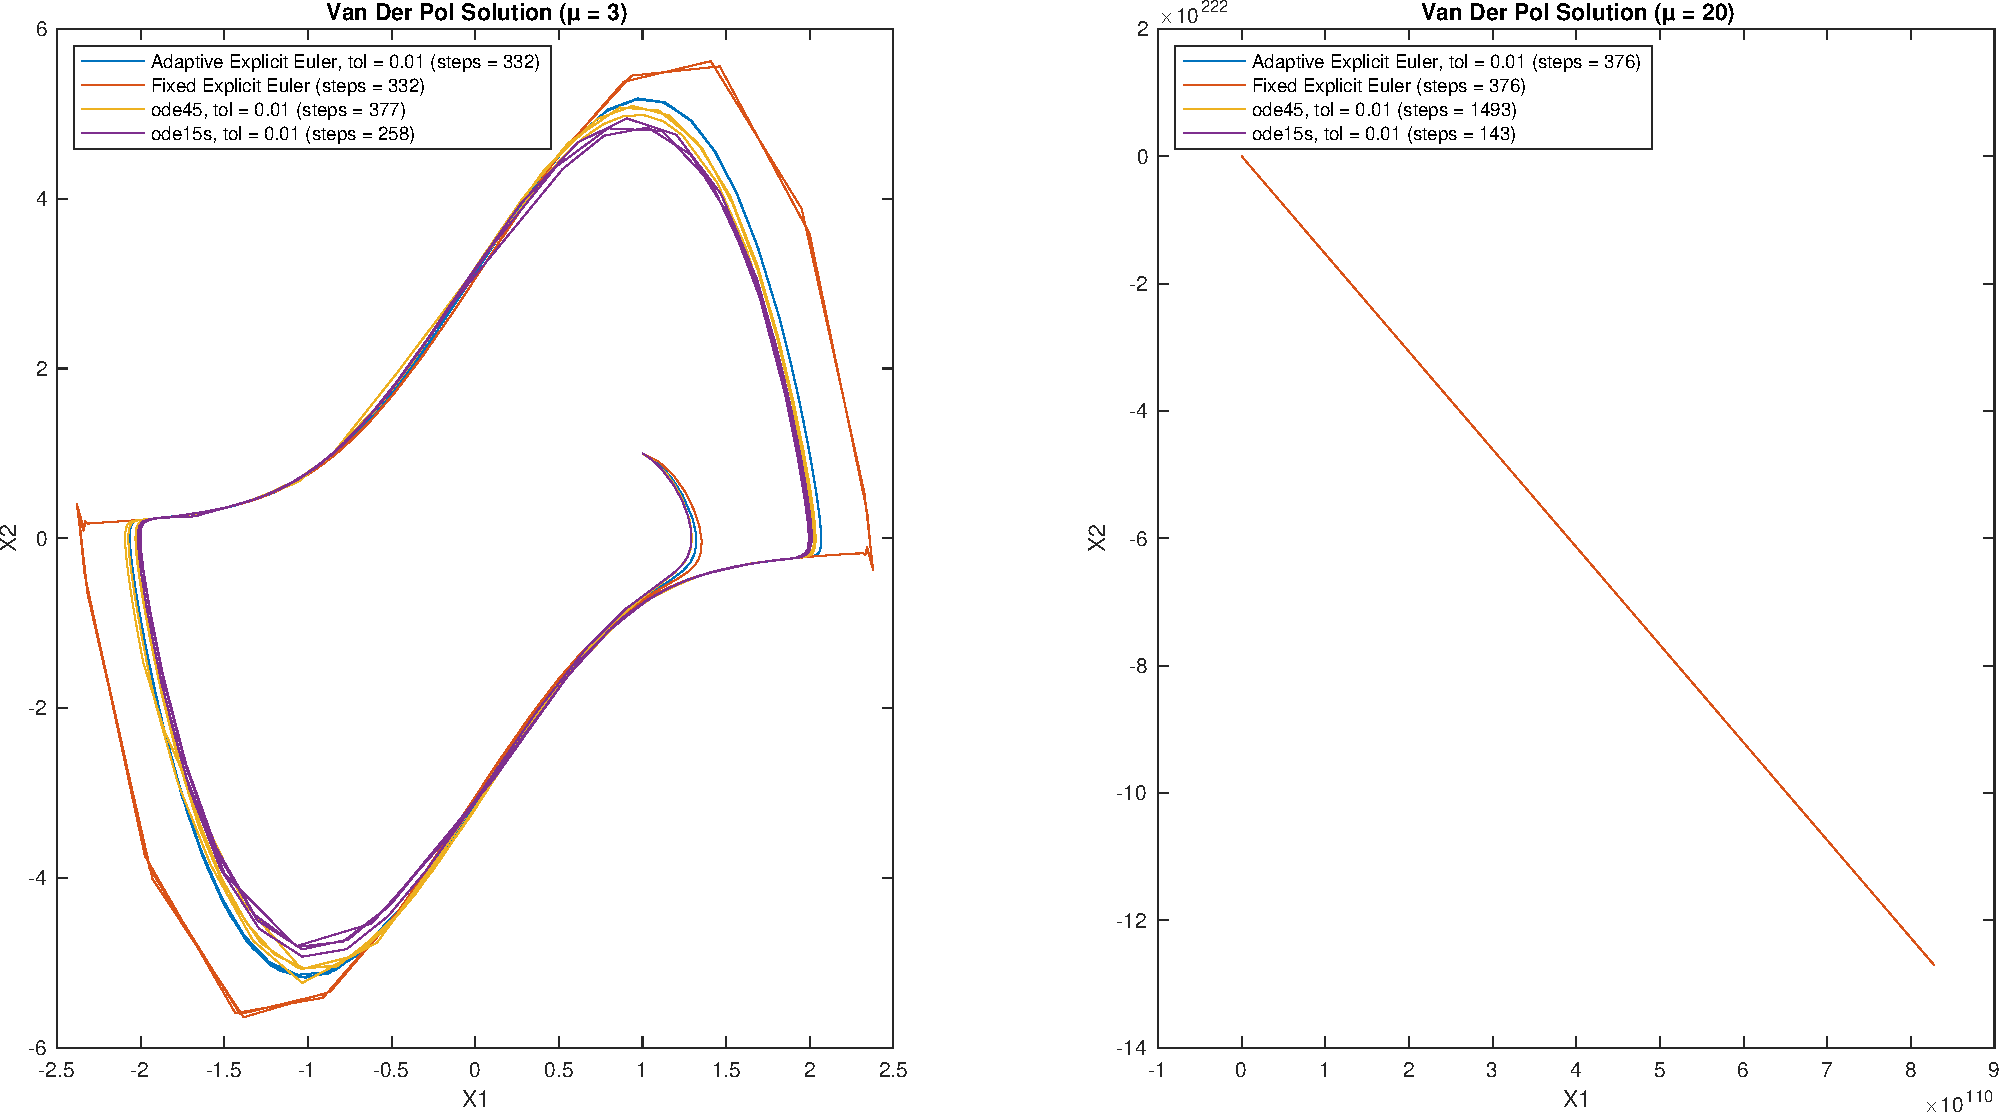
\includegraphics[width=\textwidth]{plots/2_4main_02.pdf}
    \caption{Explicit Euler method tested on the Van der Pol problem. Both an adaptive step size strategy with tolerance = 0.01 and a fixed step size strategy fixed to equal number of steps is applied.}
    \label{fig:2_4a}
\end{figure}

og yeah 

\begin{figure}[H]
    \centering
    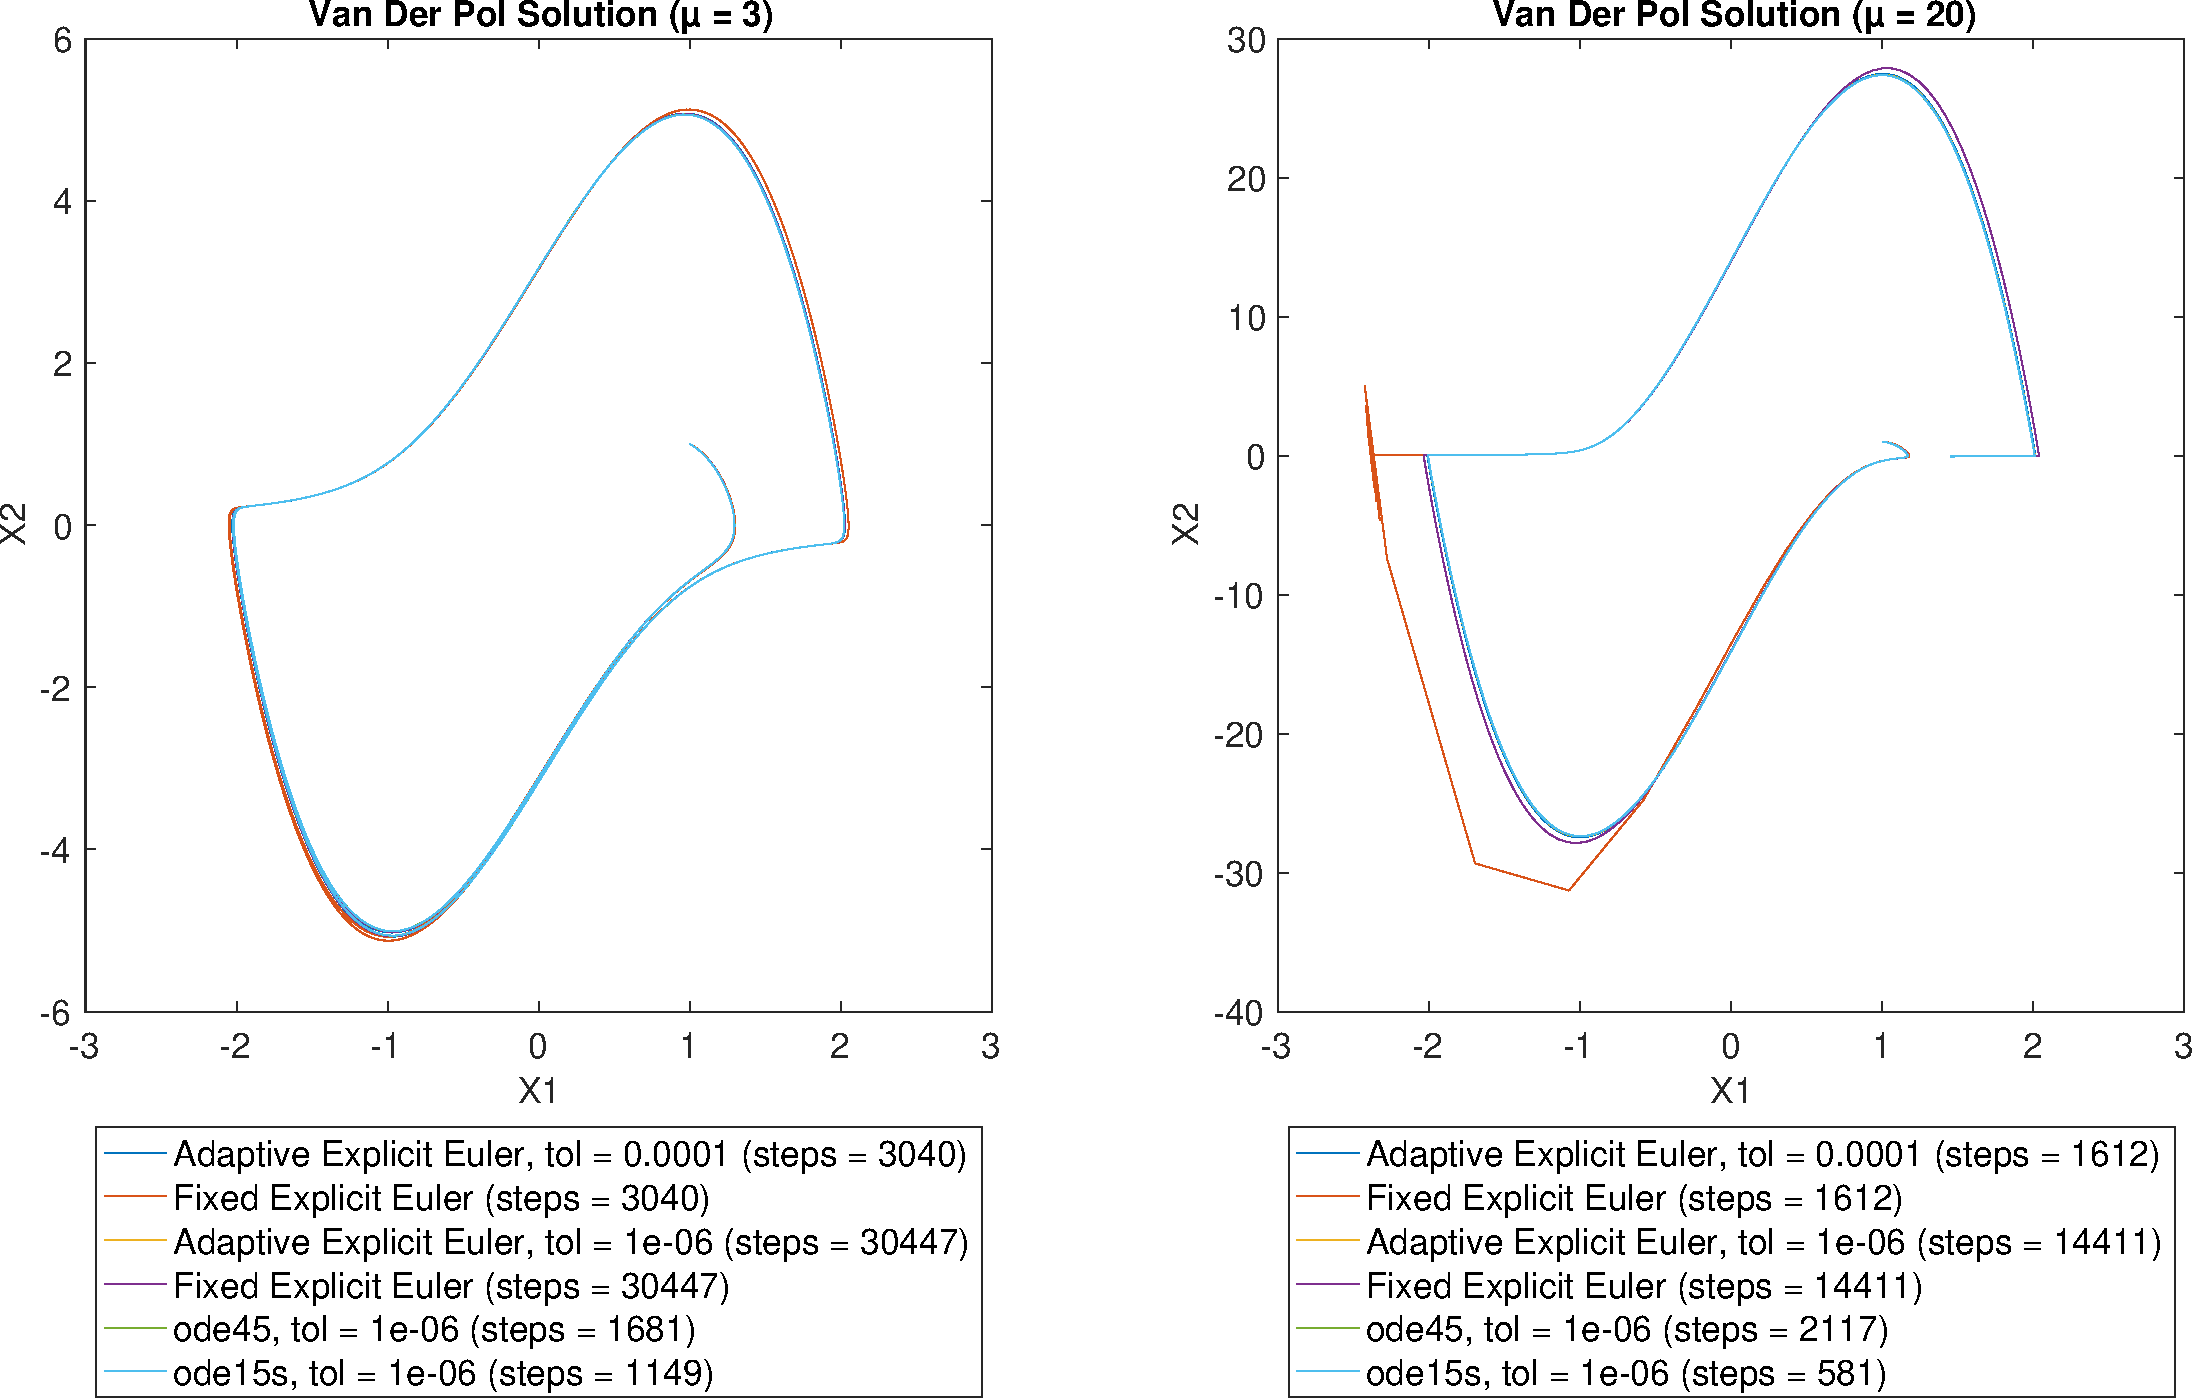
\includegraphics[width=\textwidth]{plots/2_4main_04_06.pdf}
    \caption{Explicit Euler method tested on the Van der Pol problem. Both an adaptive step size strategy with tolerances $\in \{10^{-4}, 10^{-6}\}$ and a fixed step size strategy with an equivalent number of steps is applied.}
    \label{fig:2_4b}
\end{figure}



<-- MANGLER: Noget hertil:-)
Lav du bare side-by-side fasepotræt (X1,X2) for mu = 3 (non-stiff) og mu=20(stiff)
God weekend.